%%%%%%%%%%%%%%%%%%%%%%%%%%%%%%%%%%%%%%%%%
% Beamer Presentation
% LaTeX Template
% Version 1.0 (10/11/12)
%
% This template has been downloaded from:
% http://www.LaTeXTemplates.com
%
% License:
% CC BY-NC-SA 3.0 (http://creativecommons.org/licenses/by-nc-sa/3.0/)
%
%%%%%%%%%%%%%%%%%%%%%%%%%%%%%%%%%%%%%%%%%

%----------------------------------------------------------------------------------------
%	PACKAGES AND THEMES
%----------------------------------------------------------------------------------------

\documentclass{beamer}

\mode<presentation> {

  % The Beamer class comes with a number of default slide themes
  % which change the colors and layouts of slides. Below this is a list
  % of all the themes, uncomment each in turn to see what they look like.

  %\usetheme{default}
  %\usetheme{AnnArbor}
  %\usetheme{Antibes}
  %\usetheme{Bergen}
  %\usetheme{Berkeley}
  %\usetheme{Berlin}
  %\usetheme{Boadilla}
  %\usetheme{CambridgeUS}
  %\usetheme{Copenhagen}
  %\usetheme{Darmstadt}
  %\usetheme{Dresden}
  %\usetheme{Frankfurt}
  %\usetheme{Goettingen}
  %\usetheme{Hannover}
  %\usetheme{Ilmenau}
  %\usetheme{JuanLesPins}
  %\usetheme{Luebeck}
  \usetheme{Madrid}
  %\usetheme{Malmoe}
  %\usetheme{Marburg}
  %\usetheme{Montpellier}
  %\usetheme{PaloAlto}
  %\usetheme{Pittsburgh}
  %\usetheme{Rochester}
  %\usetheme{Singapore}
  %\usetheme{Szeged}
  %\usetheme{Warsaw}

  % As well as themes, the Beamer class has a number of color themes
  % for any slide theme. Uncomment each of these in turn to see how it
  % changes the colors of your current slide theme.

  %\usecolortheme{albatross}
  %\usecolortheme{beaver}
  %\usecolortheme{beetle}
  %\usecolortheme{crane}
  %\usecolortheme{dolphin}
  %\usecolortheme{dove}
  %\usecolortheme{fly}
  %\usecolortheme{lily}
  %\usecolortheme{orchid}
  %\usecolortheme{rose}
  %\usecolortheme{seagull}
  %\usecolortheme{seahorse}
  %\usecolortheme{whale}
  %\usecolortheme{wolverine}

  %\setbeamertemplate{footline} % To remove the footer line in all slides uncomment this line
  %\setbeamertemplate{footline}[page number] % To replace the footer line in all slides with a simple slide count uncomment this line

  %\setbeamertemplate{navigation symbols}{} % To remove the navigation symbols from the bottom of all slides uncomment this line
}

\usepackage{hyperref}
\usepackage{graphicx} % Allows including images
\usepackage{booktabs} % Allows the use of \toprule, \midrule and \bottomrule in tables
\usepackage{algorithm}% http://ctan.org/pkg/algorithms
\usepackage{algpseudocode}% http://ctan.org/pkg/algorithmicx

\DeclareMathOperator*{\argmin}{arg\,min}
\DeclareMathOperator*{\argmax}{arg\,max}

%----------------------------------------------------------------------------------------
%	TITLE PAGE
%----------------------------------------------------------------------------------------

\title[TRPO]{Trust Region Policy Optimization} % The short title appears at the bottom of every slide, the full title is only on the title page

\author{Yixin Lin} % Your name
\institute[Duke] % Your institution as it will appear on the bottom of every slide, may be shorthand to save space
{
  Duke University \\ % Your institution for the title page
  \medskip
  \textit{yixin.lin@duke.edu} % Your email address
}
\date{March 28, 2017} % Date, can be changed to a custom date

\begin{document}

\begin{frame}
  \titlepage % Print the title page as the first slide
\end{frame}

\begin{frame}
  \frametitle{Overview} % Table of contents slide, comment this block out to remove it
  \tableofcontents % Throughout your presentation, if you choose to use \section{} and \subsection{} commands, these will automatically be printed on this slide as an overview of your presentation
\end{frame}

%----------------------------------------------------------------------------------------
%	PRESENTATION SLIDES
%----------------------------------------------------------------------------------------

%------------------------------------------------
% \section{First Section} % Sections can be created in order to organize your presentation into discrete blocks, all sections and subsections are automatically printed in the table of contents as an overview of the talk
%------------------------------------------------

% \subsection{Subsection Example} % A subsection can be created just before a set of slides with a common theme to further break down your presentation into chunks

\section{Preliminaries}

\subsection{Markov Decision Processes}


\begin{frame}
\frametitle{Introduction}
\begin{itemize}
  \item Reinforcement learning is the problem of \textit{sequential decision making in dynamic environment}
  \item Goal: capture the most important aspects of an agent making decisions
    \begin{itemize}
      \item Input (sensing the state of the environment)
      \item Action (choosing to affect on the environment)
      \item Goal (prefers some states of the environment over others)
    \end{itemize}
  \item This is \textit{incredibly} general
  \item Examples
    \begin{itemize}
      \item Robots (and their components)
      \item Games
      \item Better A/B testing
    \end{itemize}
\end{itemize}
\end{frame}

\begin{frame}
  \frametitle{The Markov Decision Process (MDP)}
  \begin{itemize}
    \item $S$: set of possible \textbf{states} of the environment
      \begin{itemize}
        \item $p(s_{init}), s_{init} \in S$: a distribution over initial state
        \item Markov property: we assume that the current state summarizes everything we need to remember
      \end{itemize}
    \item $A$: set of possible \textbf{actions}
      \begin{itemize}
        \item $P(s_{new} | s_{old}, a)$: state transitions, for each state $s$ and action $a$
      \end{itemize}
    \item $R: S \rightarrow \mathbb{R}$: \textbf{reward}
      \begin{itemize}
        \item $\gamma \in [0,1]$: discount factor
      \end{itemize}
  \end{itemize}
\end{frame}


\subsection{Policy iteration}

\begin{frame}
  \frametitle{Policies and value functions}
  \begin{itemize}
    \item $\pi$: a policy (what action to do, given a state)
    \item Return: (possibly discounted) sum of future rewards $r_t + \gamma r_{t+1} + \gamma^2 r_{t+2} \ldots$
    \item Performance of policy: $\eta(\pi) = \mathbb{E} [\text{return}]$
    \item $V^\pi(s) = E_\pi[\text{return} \mid s]$
      \begin{itemize}
        \item How good is a state, given a policy?
      \end{itemize}
    \item $Q^\pi(s, a) = E_\pi[\text{return} \mid s, a]$
      \begin{itemize}
        \item How good is an action at a state, given a policy?
      \end{itemize}
      % \item More realistic: Partially Observed MDPs (POMDPs), where state is not directly observed but affects observations
      %   \begin{itemize}
      %     \item Hidden-state transitions $P(s_{new} | s_{old}, a)$
      %     \item Observation based on hidden state $y \sim P(y|s)$
      %   \end{itemize}
  \end{itemize}
\end{frame}


\begin{frame}
  \frametitle{Policy iteration}
  \begin{itemize}
    \item Assume perfect model of MDP
    \item Alternate between the following until convergence
      \begin{itemize}
        \item Evaluating the policy (computing $V^\pi$)
          \begin{itemize}
            \item For each state $s$, $V(s) = \mathbb{E} [\sum_{s', r} r + \gamma V(s')]$
            \item Repeat until convergence (or just once for \textit{value iteration})
          \end{itemize}
        \item Setting policy to be greedy ($\pi(s) = \argmax_a \mathbb{E} [r + \gamma V^\pi (s')]$)
      \end{itemize}
    \item Guaranteed convergence (for both policy and value iteration)
  \end{itemize}
\end{frame}

\subsection{Policy gradients}

\begin{frame}
  \frametitle{Policy gradients}
  \begin{itemize}
    \item Policy iteration scales very badly: have to repeatedly evaluate policy on all states
    \item Parameterize policy $a \sim \pi | \theta$
    \item We can sample instead
  \end{itemize}
\end{frame}
\begin{frame}
  \frametitle{Policy gradients}
  \begin{itemize}
    \item Sample a lot of \textit{trajectories} (simulate your environment under the policy) under the current policy
    \item Make good actions more probable
      \begin{itemize}
        \item Specifically, estimate gradient using \textit{score function gradient estimator}
        \item For each trajectory $\tau_i$, $\hat{g}_i = R(\tau_i) \nabla_\theta \log p(\tau_i|\theta)$
        \item Intuitively, take the gradient of log probability of the trajectory, then weight it by the final reward
        \item Reduce variance by temporal structure and other tricks (e.g. baseline)
          \begin{itemize}
            \item Replace reward by the advantage function $A_\pi = Q_\pi(s,a) - V_\pi(s)$
            \item Intuitively, how much better is the action we picked over the average action?
          \end{itemize}
      \end{itemize}
    \item Repeat
  \end{itemize}
\end{frame}

\begin{frame}
  \frametitle{Vanilla policy gradient algorithm/REINFORCE}
  \begin{algorithmic}
    \State Initialize policy $\pi | \theta$
    \While{gradient estimate has not converged}
    \State Sample trajectories using $\pi$
    \For{each timestep}
    \State Compute return and advantage estimate
    \EndFor
    \State Refit optimal baseline
    \State Update the policy using gradient estimate $\hat{g}$
    \EndWhile
  \end{algorithmic}
\end{frame}

\begin{frame}
  \frametitle{Connection to supervised learning}
  \begin{itemize}
    \item Minimizing $L(\theta) = \sum_t \log \pi(a_t | s_t ; \theta) \hat{A_t}$
      \begin{itemize}
        \item In the paper, they use cost functions instead of reward functions
      \end{itemize}
    \item Intuitively, we have some parameterized policy (``model'') giving us a distribution over actions
    \item We don't have the correct action (``label''), so we just use the reward at the end as our label
    \item We can do better. How do we do credit assignment?
      \begin{itemize}
        \item Baseline (roughly encourage half of the actions, not just all of them)
        \item Discounted future reward (actions affect near-term future), etc.
      \end{itemize}
  \end{itemize}
\end{frame}

\section{TRPO}

\subsection{Kakade \& Langford}

\begin{frame}
  \frametitle{Kakade \& Langford: conservative policy iteration}
  \begin{itemize}
    \item ``A useful identity'' for $\eta_{\tilde{\pi}}$, the expected discounted cost of a new policy $\tilde{\pi}$
    \item $\eta(\tilde{\pi}) = \eta(\pi) + \mathbb{E} [ \sum_{t=0} \gamma^t A_\pi (s_t, a_t)] = \eta(\pi) + \sum_s \rho_{\tilde{\pi}} (s) \sum_a \tilde{\pi} (a|s) A_\pi (s,a)$
    \item Intuitively: the expected return of a new policy is the expected return of the old policy, plus how much better the new policy is at each state
    \item Local approximation: switch out $\rho_{\tilde{\pi}}$ for $\rho_\pi$, since we only have the state visitation frequency for the old policy, not the new policy
      \begin{itemize}
        \item $L_\pi (\tilde{\pi}) = \eta(\pi) + \sum_s \rho_\pi (s) \sum_a \tilde{\pi} (a|s) A_\pi (s,a)$
      \end{itemize}
    \item Kakade \& Langford proved that optimizing this local approximation is good for small step sizes, but for mixture policies only
  \end{itemize}
\end{frame}

\subsection{Natural policy gradients}
\begin{frame}
  \frametitle{Natural policy gradients}
  \begin{itemize}
    \item In this paper, they prove that $\eta(\tilde{\pi}) \leq L_\pi(\tilde{\pi}) + CD_{KL}^{\max} (\pi, \tilde{\pi})$, $C$ is a constant dependent on $\gamma$
    \item Intuitively, we optimize the approximation, but regularize with the KL divergence between old and new policy
    \item Algorithm called the natural policy gradient
    \item Problem: choosing hyperparameter $C$ is difficult
  \end{itemize}
\end{frame}

\subsection{Overview of TRPO}
\begin{frame}
  \frametitle{Overview of TRPO}
  \begin{itemize}
    \item Instead of adding KL divergence as a cost, simply use it as an optimization constraint
    \item TRPO algorithm: minimize $L_\pi(\tilde{\pi})$, constraint that $D_{KL}^{\max} \leq \delta$ for some easily-picked hyperparameter $\delta$
  \end{itemize}
\end{frame}

\subsection{Practice}

\begin{frame}
  \frametitle{Practical considerations}
  \begin{itemize}
    \item How do we sample trajectories?
      \begin{itemize}
        \item Single-path: simply run each sample to completion
        \item ``Vine'': for each sampled trajectory, pick random states along the trajectory and perform small rollout
      \end{itemize}
    \item How do we compute gradient? Use conjugate gradient algorithm followed by line search
  \end{itemize}
\end{frame}

\begin{frame}
  \frametitle{Algorithm}
  \begin{algorithmic}
    \While{gradient not converged}
      \State Collect trajectories (either single-path or vine)
      \State Estimate advantage function
      \State Compute policy gradient estimator
      \State Solve quadratic approximation to $L(\pi_\theta)$ using CG
      \State Rescale using line search
      \State Apply update
    \EndWhile
  \end{algorithmic}
\end{frame}

\subsection{Experiments}

\begin{frame}
  \frametitle{Experiments - MuJoCo robotic locomotion}

  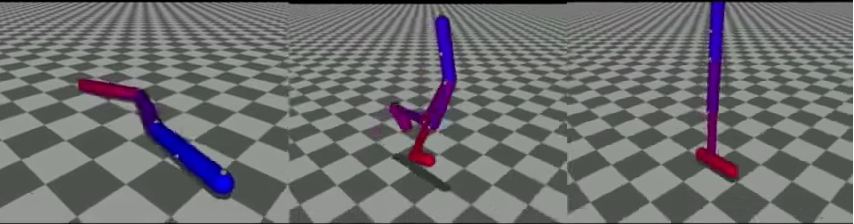
\includegraphics[width=0.8\textwidth]{mujoco.png}

  \begin{itemize}
    \item \href{https://www.youtube.com/watch?v=KJ15iGGJFvQ}{Link to demonstration}
    \item Same $\delta$ hyperparameter across experiments
  \end{itemize}

\end{frame}

\begin{frame}
  \frametitle{Experiments - MuJoCo learning curves}
  \centering
  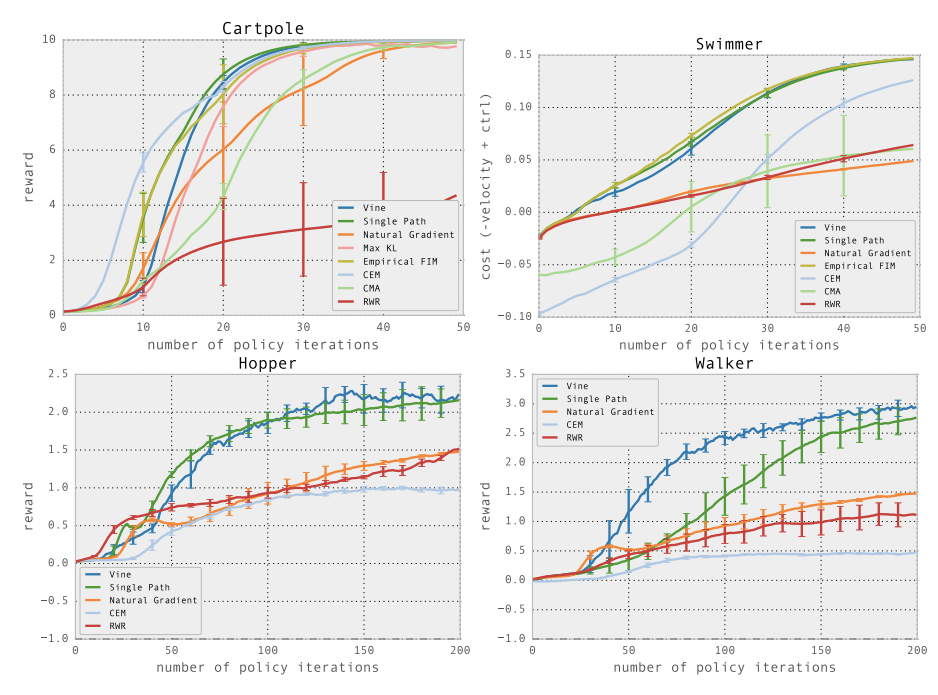
\includegraphics[width=0.7\textwidth]{experiments.png}

  \begin{itemize}
    \item \href{https://www.youtube.com/watch?v=KJ15iGGJFvQ}{Link to demonstration}
    \item Same $\delta$ hyperparameter across experiments
  \end{itemize}
\end{frame}

\begin{frame}
  \frametitle{Experiments - Atari}
  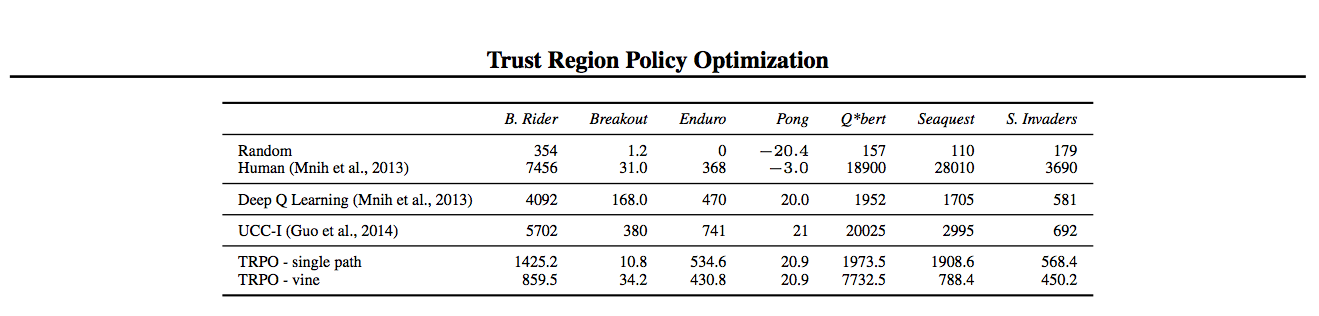
\includegraphics[width=\textwidth]{games_table.png}

  \begin{itemize}
    \item Not always better than previous techniques, but consistently decent
    \item Very little problem-specific engineering
  \end{itemize}
\end{frame}

\begin{frame}
  \frametitle{Takeaway}
  \begin{itemize}
    \item TRPO is a good default policy gradient technique which scales well and has minimal hyperparameter tuning
    \item Just use KL constraint on gradient approximator
  \end{itemize}
\end{frame}

%------------------------------------------------

%------------------------------------------------

\section{References}

\begin{frame}
  \frametitle{References}
  \footnotesize{
    \begin{thebibliography}{99} % Beamer does not support BibTeX so references must be inserted manually as below
      \bibitem[]{} RS Sutton. Introduction to reinforcement learning
      \bibitem[]{} Kakade and Langford. Approximately optimal approximate reinforcement learning
      \bibitem[]{} Schulman et al. Trust Region Policy Optimization
      \bibitem[]{} Schulman, Levine, Finn. Deep Reinforcement Learning course: \href{http://rll.berkeley.edu/deeprlcourse/}{link}
      \bibitem[]{} Andrej Karpathy. Deep Reinforcement Learning: From Pong to Pixels: \href{http://karpathy.github.io/2016/05/31/rl/}{link}
      \bibitem[]{} Trust Region Policy Optimization summary: \href{https://jmk.pe.kr/media/attachments/5bcf0aca45da310a434bbc093799c85e/trpo.pdf}{link}
  \end{thebibliography}
}
\end{frame}

%------------------------------------------------

\begin{frame}
  \Huge{\centerline{Thanks!}}
  
  \Large{\centerline{Link to presentation: \href{http://yixinlin.net/trpo}{yixinlin.net/trpo}}}
\end{frame}

%----------------------------------------------------------------------------------------

\end{document} 
